\documentclass[a4paper, 11pt, twocolumn]{article}

\usepackage[czech]{babel}
\usepackage[utf8]{inputenc}
\usepackage[IL2]{fontenc}
\usepackage[left=1.5cm, top=2.5cm, text={18cm, 25cm}]{geometry}

\usepackage{times}
\usepackage{amsthm}
\usepackage{amssymb}
\usepackage{amsmath}
\usepackage{stackrel}
\usepackage{graphicx}

\graphicspath{{./img/}}



\begin{document}

	\begin{titlepage}
		\begin{center}
			\begin{center}
			
\includegraphics[scale=0.15]{logo_cz.png} \\
			\end{center}
			\vspace{\stretch{0.382}} 
			\huge {Technická zpráva k projektu} \\
			\Large {Tvorba uživatelských rozhraní} \\
			\vspace{\stretch{0.618}}
		\end{center}

		\Large{\hfill Vojtěch Kališ (xkalis03)} \\
		\Large{2021 \hfill Jan Lutonský (xluton02)}
	\end{titlepage}
	



	\twocolumn[{\centering{\LARGE \textbf{\underline{Školní administrativní systém}}\par}}
	\par\vspace*{0.8cm}]

	\section*{\large{Podrobná specifikace zadání}}
	\vspace*{-0.2cm}
	Pod pojmem 'Školní administrativní systém' je obecně zapotřebí si představit databázi studentů, zaměstnanců školy a školního majetku jejíž hlavními 
	uživateli jsou administrativní pracovníci, kteří mají za účel převážně vkládat do systému informace, a poté učitelé, kteří naopak chtějí dané informace 
	zobrazovat. V našem návrhu řešení jsme se zaměřili převážně na část systému zabývající se vpisováním/zobrazováním informací o studentech ,jelikož to je 
	právě ta část jenž je využívána nejvíce, a navýše i uživateli u nichž se počítá s méně zkušenostmi v oblasti navigace technologiemi a kde obecně správný a 
	hlavně přehledný návrh GUI bývá nejkritičtějším bodem v rámci systémového návrhu. Dále jsme si ji rozdělili na rozhraní pro administrativní pracovníky a 
	rozhraní pro učitele. I takhle zadané téma ovšem v sobě zahrnuje příliš veliké množství prvků a tak byla realizace limitována na následující funkce: \\
	\vspace*{0.2cm} \\
	\noindent\textbf{Návrh pro administrativní pracovníky} 
	\begin{itemize}
		\item ...
		\vspace{-0.2cm}
		\item ...
		\vspace{-0.2cm}
		\item ...
		\vspace{-0.2cm}
		\item ...
		\vspace{-0.2cm}
		\item ...
	\end{itemize}
	\vspace*{0.2cm}

	\noindent\textbf{Návrh pro učitele} 
	\begin{itemize}
		\item Interaktivní hlavička odkazující na domovskou stránku
		\vspace{-0.2cm}
		\item Přehledný toolbar se všemi důležitými odkazy
		\vspace{-0.2cm}
		\item Logika měnění obsahu stránky podle posledního odkazu, jenž byl rozkliknut
		\vspace{-0.2cm}
		\item Tabulka obsahující seznam studentů, zobrazující se pouze po rozkliknutí odkazu 'Databáze'
		\vspace{-0.2cm}
		\item Simplistické vyhledávací okénko se zabudovanou logikou vyhledávání studenta podle jména, ID či hudebního nástroje na který je zapsán
		\vspace{-0.2cm}
		\item Tlačítko obsaženo v rámci tabulky studentů, po jehož rozkliknutí se zobrazí podrobnější informace o studentovi
		\vspace{-0.2cm}
		\item Základ možnosti přihlášení se pomocí vlastního ID a hesla (bez implementace logiky)
	\end{itemize}


	\vspace*{\fill}
	\newpage


	\section*{\large{Návrh architektury a GUI}}
	\vspace*{-0.2cm}
	Jak již bylo zmíněno v předešlé sekci, se systémem pracují dvě skupiny uživatelů, a to administrační pracovníci a učitelé. Administrační pracovníci mají 
	zkušenosti s prací na počítači a většínu dne tráví editací údajů v systému. Učitelé na druhou stranu jsou většinou starší lidé a mají problém při práci s 
	počítačem, a proto si zvykli se systémem spíše nepracovat vůbec a veškerou svou práci převedli na administrativní pracovníky. Učitelé ze systému potřebují 
	převážně jen číst informace. Návrhy pro GUI pro obě skupiny uživatelů jsou tedy zásadně velice rozlišné a tak se ponouká varianta vytvoření jednoho návrhu 
	zaměřujícího se více na funkci a druhého který bude zaměřen naopak spíše na design a usnadnění práce s finálním produktem, přičemž je samozřejmě i 
	zapotřebí aby spolu oba designy komunikovaly, pokud možno jednolitě, proto jsme se rozhodli rozdělit architekturu a zároveň i vlastní práci v týmu do 
	těchhle bodů: \\
	\vspace*{-0.6cm}
	\begin{itemize}
		\item Návrh GUI pro administrativní pracovníky
		\vspace{-0.2cm}
		\item Návrh GUI pro učitele
		\vspace{-0.2cm}
		\item Zajištění vzájemné komunikace obou návrhů (jehož realizace je popsána v následující sekci)
	\end{itemize}
	\vspace*{0.4cm}

	\noindent\textbf{Předběžný návrh GUI pro učitele lze vidět v následujícím obrázku} 
	\begin{center}
	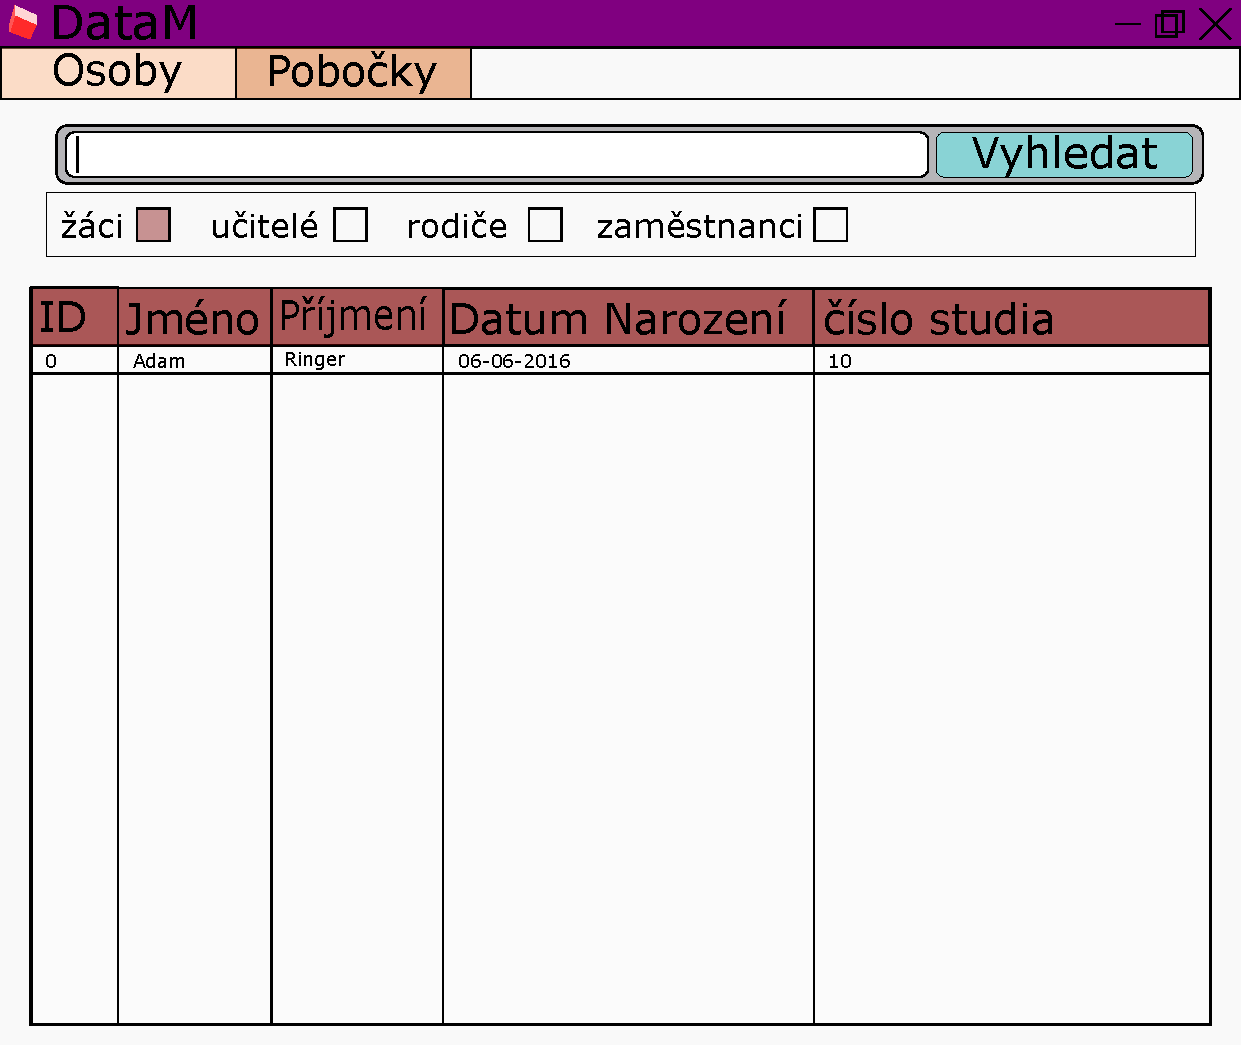
\includegraphics[width=0.5\textwidth]{GUI.pdf}
	\end{center}


	\vspace*{\fill}
	\clearpage


	\section*{\large{Popis použitých nástrojů a implementace}}
	\vspace*{-0.2cm}
	\vspace*{0.3cm}
	\noindent\textbf{\underline{Společně byly použity: }} \\
	\noindent\textbf{Flask: } Pythonový webový microframework s možností výberu frameworku pro objektovou práci s databází \\
	\noindent\textbf{SQLAlchemy: } Námi vybraný framework pro Flask. Jedná se o objektovou vrstvu nad databázovou knihovnou, která umožňuje pracovat s 
	tabulkami jako s kolekcemi objektů \\
	\vspace*{0.5cm} \\
	\noindent\textbf{\underline{V GUI pro administrativní pracovníky byly použity: }} \\
	\noindent\textbf{x: } ... \\
	\noindent\textbf{x: } ... \\
	\noindent\textbf{x: } ... \\
	\vspace*{0.5cm} \\
	\noindent\textbf{\underline{V GUI pro učitele byly použity: }} \\
	\noindent\textbf{HTML: } pro markup, vytváření základních bloků a spojování celků do závěrečné podoby z vizuálního hlediska \\
	\noindent\textbf{CSS: } pro globální zajištění kontroly layoutu a vzhledu jednotlivých HTML bloků a shrnutí těchto stylů do jednoho souboru \\
	\noindent\textbf{JavaScript: } pro vytváření funkcí manipulující s HTML prvky a pro zajištění čtení dat ve formátu JSON ze serveru, jejich následného 
	přetypování a dynamického vytváření HTML bloků \\
	\vspace*{0.5cm} \\
	\noindent Veškeré dependencies či jejich instalace jsou dále také popsány v jednotlivých \textit{README.md} souborech u jednotlivých implementací obou 
	GUI, společně s návodem na jejich zprovoznění. Je také vyžadována případná instalace buď Python 2.7 nebo Python 3.5 či novější. \\
	

	\vspace*{\fill}
	\clearpage


	\section*{\large{Screenshoty výsledných aplikací}}
	\vspace*{-0.2cm}
	


\end{document}